\documentclass{article}

\usepackage{graphicx}
\usepackage{tikz}
\usepackage{tikzsymbols}
\usetikzlibrary{calc,patterns,shapes.geometric}
\pagestyle{empty}
\usepackage[margin=0pt]{geometry}
\geometry{papersize={14in,12in}}

\def\centerarc[#1](#2)(#3:#4:#5){\draw[#1] ($(#2)+({#5*cos(#3)},{#5*sin(#3)})$) arc (#3:#4:#5);}

\begin{document}
	\begin{figure}
		\centering
		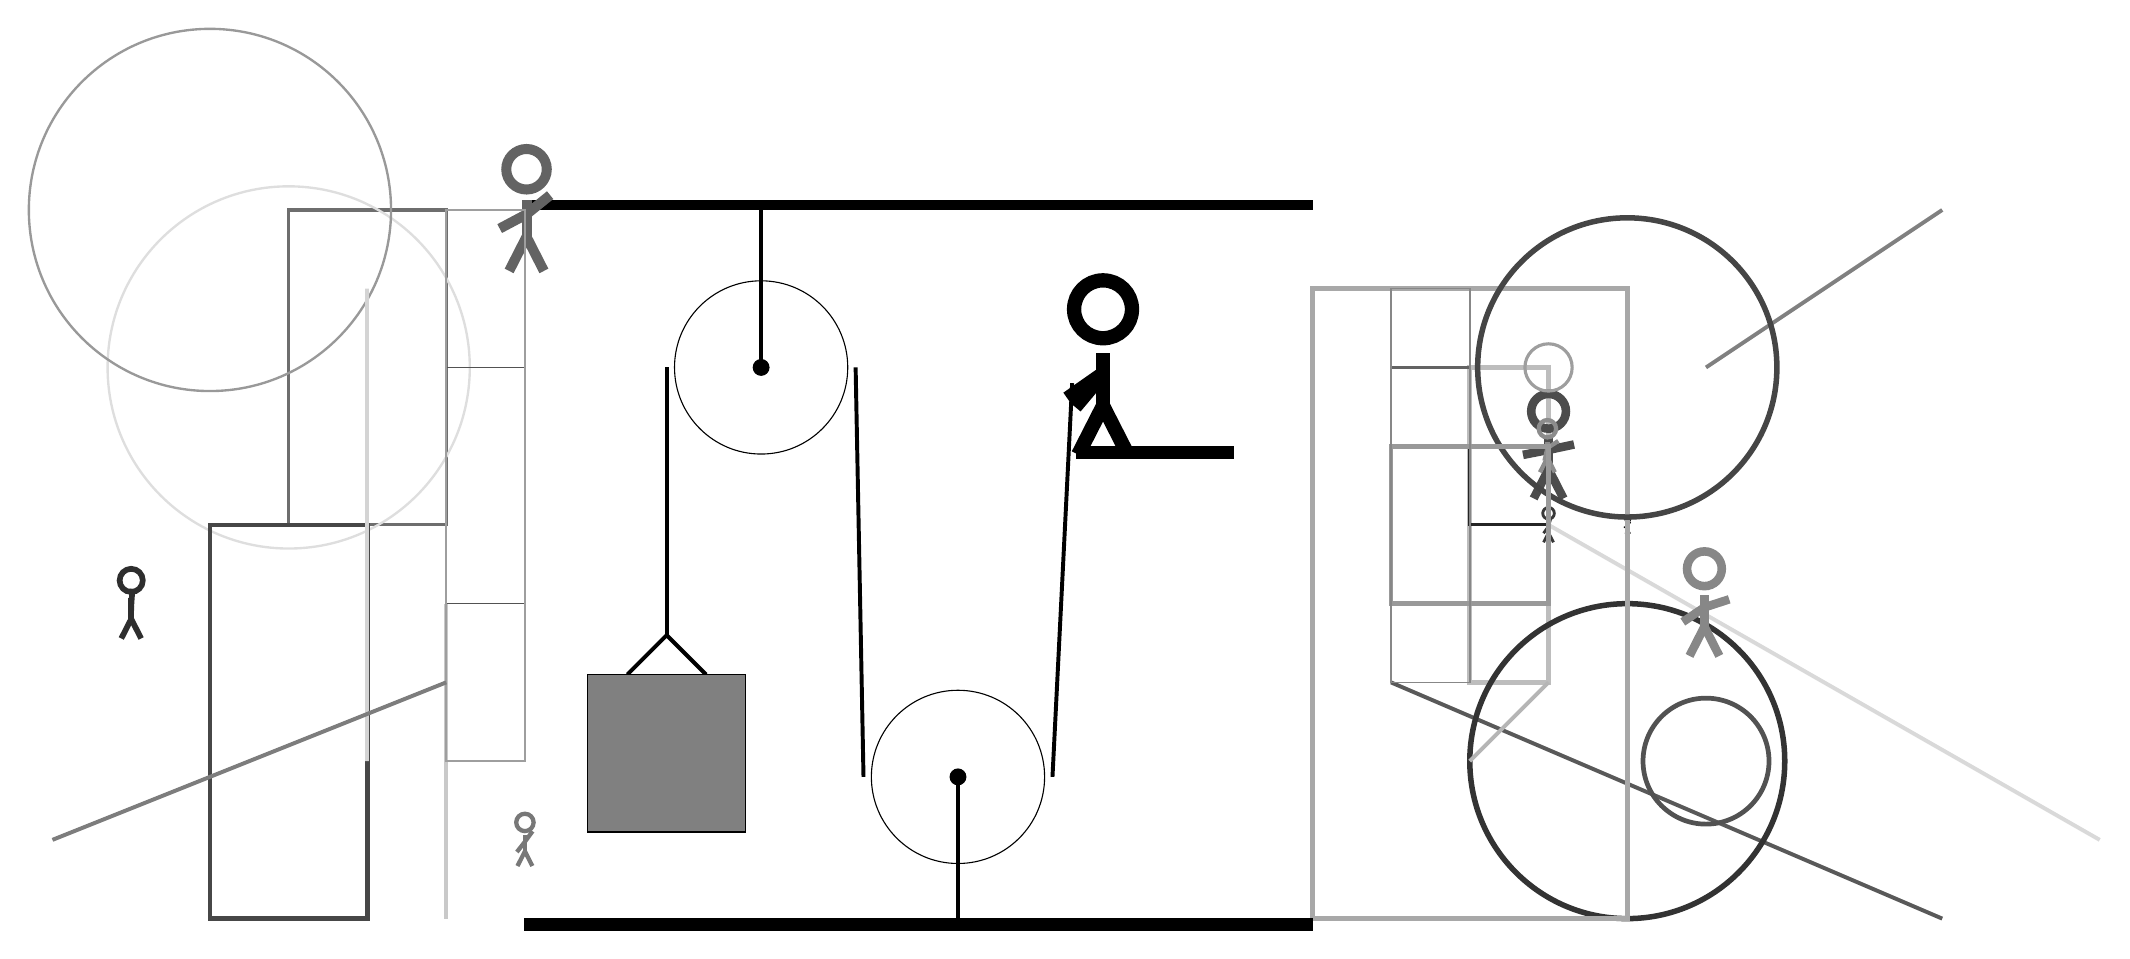
\begin{tikzpicture}
			%%%%% START %%%%%
			
			\draw[fill=black] (-2, 9) rectangle (8, 9.125);
			
			\draw (3.5, 1.8) circle (1.1);
			\draw[fill=black] (3.5, 1.8) circle (0.1);
			\draw[line width=0.5mm] (3.5, 1.8) -- (3.5, 0);
			
			\draw (1, 7) circle (1.1);
			\draw[fill=black] (1, 7) circle (0.1);
			\draw[line width=0.5mm] (1, 9) -- (1, 7);
			
			\draw[line width=0.5mm](-0.7, 3.1) --  (-0.2, 3.6) -- (0.3, 3.1);
			\draw[fill=black!50] (-1.2, 3.1) rectangle (0.8, 1.1);
			
			\draw[line width=0.5mm](-0.2, 7) -- (-0.2, 3.6);
			\centerarc[line width=0.5mm](1, 7)(180:0:1.2000000000000002)
			\draw[line width=0.5mm](2.2, 7) -- (2.3, 1.8);
			\centerarc[line width=0.5mm](3.5, 1.8)(180:360:1.2000000000000002)
			\draw[line width=0.5mm](4.7, 1.8) -- (4.95, 6.8);
			
			\node at (5.3, 7) {\Strichmaxerl[10][35][-130]};
			\draw[fill=black] (5, 6) rectangle (7, 5.85);
			
			\draw[line width=0.6mm, color=black!26] (10, 3) rectangle (11, 7);
			
			\node[line width=0.5mm, color=black!70] at (11, 6) {\Strichmaxerl[6][11][12]};
			\draw[line width=0.5mm, color=black!21](-3, 4) -- (-3, 0);
			\draw[line width=0.4mm, color=black!57] (-3, 9) rectangle (-5, 5);
			
			\draw[line width=0.3mm, color=black!61] (10, 8) rectangle (9, 7);
			\draw [line width=0.3mm, color=black!13](-5, 7) circle (2.3);
			
			\draw[line width=0.2mm, color=black!68] (-2, 4) rectangle (-3, 7);
			\node[line width=0.5mm, color=black!45] at (11, 6) {\Strichmaxerl[3][77][33]};
			\draw[line width=0.5mm, color=black!15](11, 5) -- (18, 1);
			
			\draw[line width=0.5mm, color=black!65](9, 3) -- (16, 0);
			\draw [line width=0.7mm, color=black!80](12, 2) circle (2.0);
			
			\node[line width=0.5mm, color=black!61] at (-2, 9) {\Strichmaxerl[7][28][39]};
			\node[line width=0.5mm, color=black!82] at (-7, 4) {\Strichmaxerl[4][89][86]};
			\draw[line width=0.5mm, color=black!29](11, 3) -- (10, 2);
			\node[line width=0.4mm, color=black!95] at (12, 5) {\Strichmaxerl[1][28][51]};
			\draw [line width=0.3mm, color=black!40](-6, 9) circle (2.3);
			
			\draw[line width=0.6mm, color=black!72] (-4, 5) rectangle (-6, 0);
			
			\draw[line width=0.3mm, color=black!38] (-2, 2) rectangle (-3, 9);
			\node[line width=0.2mm, color=black!47] at (13, 4) {\Strichmaxerl[6][34][18]};
			\draw[line width=0.5mm, color=black!50](13, 7) -- (16, 9);
			\node[line width=0.4mm, color=black!53] at (-2, 1) {\Strichmaxerl[3][52][54]};
			
			\draw [line width=0.4mm, color=black!38](11, 7) circle (0.3);
			
			\draw[line width=0.7mm, color=black!34] (8, 8) rectangle (12, 0);
			\draw[line width=0.5mm, color=black!17] (-4, 8) rectangle (-4, 2);
			\draw[line width=0.4mm, color=black!86] (10, 6) rectangle (11, 5);
			
			\draw [line width=0.6mm, color=black!68](13, 2) circle (0.8);
			\node[line width=0.6mm, color=black!78] at (11, 5) {\Strichmaxerl[2][55][74]};
			\draw[line width=0.5mm, color=black!51](-3, 3) -- (-8, 1);
			
			\draw [line width=0.7mm, color=black!73](12, 7) circle (1.9);
			
			\draw[line width=0.6mm, color=black!40] (9, 4) rectangle (11, 6);
			\draw[line width=0.2mm, color=black!47] (10, 3) rectangle (9, 8);
			
			
			\draw[fill=black] (-2, 0) rectangle (8, -0.15);
			
			%%%%% END %%%%%
		\end{tikzpicture}
	\end{figure}	
\end{document}